\documentclass[10pt]{article}
\usepackage{fancyhdr}
\usepackage{listings}
\usepackage{tikz}
\usetikzlibrary{decorations.pathreplacing,shapes,arrows,positioning}

\setlength{\textwidth}{7.25in}
\setlength{\textheight}{9in}
\setlength{\topmargin}{-0.75in}
\setlength{\oddsidemargin}{-0.5in}
\setlength{\evensidemargin}{-0.5in}
\setlength{\headheight}{59pt}

\setlength\parindent{0pt}

\fancyhead[R]{CS 111C Jessica Masters\\
				Homework 7\\
				Chapter 16: Searching\\
				Chapter 19: Hashing\\
				Richard Szeto}
				
\pagestyle{fancy}

\lstset{language=Java}

\begin{document}

\begin{center}
	\large{\textbf{Homework 7}}
\end{center}

\section{Part I: Searching}
I have provided a driver program that you can use to test your solutions to \#1-2 and 5-7. I have also provided a modified \texttt{Alist} class.
	
	\begin{itemize}
		\item You must use this method \texttt{Alist} class - not previous versions from other assignments.
		
		\item I have commented the places in \texttt{Alist} where your code should go. Remove the placeholder \texttt{return} statements and write your code in those places.
		
		\item As always, the use of the driver program is optional and you might want to include additional checks to make sure your methods work properly
	\end{itemize}
	
	\begin{enumerate}
		\item[1.] Revise the recursive method \texttt{search}, as given in Segment 16.6, so that it looks at the last entry in the array instead of the first one.
		
			\begin{itemize}
				\item You can access \texttt{list} directly in your method
			\end{itemize}
			
			\vspace{0.5cm}
			Refer to AList.java
			\vspace{0.5cm}
		
		\item[2.] When searching a sorted array sequentially, you can ascertain that a given item does not appear in the array without searching the entire array. For example, if you search the array
		
		\vspace{0.5cm}
		[2 5 7 9]
		
		\vspace{0.5cm}
		for 6, you can use the approach described in Segment 16.8. That is, you compare 6 to 2, then to 5, and finally to 7. Since you did not find 6 after comparing it to 7, you do not have to look further, because the other elements in the array are greater than 7 and therefore cannot equal 6. Thus, you do not simply ask whether 6 equals an array element, you also ask whether it is greater than the element. Since 6 is greater than 2, you continue the search. Likewise 5. Since 6 is less than 7, you have passed the point in the array where 6 would have had to occur, so 6 is not in the array.
		
			\begin{itemize}
				\item You can access \texttt{list} directly in your method.			
			\end{itemize}
			
			\begin{enumerate}
				\item Write an iterative method \texttt{contains} to take advantage of these observations when searching a sorted array sequentially.
					
					\vspace{0.5cm}
					Refer to AList.java
					\vspace{0.5cm}
				
				\item Write a recursive method \texttt{search} that a method \texttt{contains} can call to take advantage of these observations when searching a sorted array sequentially.
					
					\begin{itemize}
						\item You may need more than one method to accomplish this recursively.
					\end{itemize}
					
					\vspace{0.5cm}
					Refer to AList.java
					\vspace{0.5cm}
			\end{enumerate}
		
		\item[4.] Trace the method \texttt{binarySearch}, as given in Segment 16.13, when searching for 4 in the following array of values:
		
			\vspace{0.5cm}
			[5 8 10 13 15 20 22 26 30 31 34 40]
			
			\vspace{0.5cm}
			Repeat the trace when searching for 34.
				
				\begin{itemize}
					\item List the values of \texttt{first}, \texttt{last}, and \texttt{mid} for each call to \texttt{binarySearch}
				\end{itemize}
				
			\vspace{0.5cm}
			\begin{tikzpicture}
				\foreach \i [count=\n] in {5,8,10,13,15,20,22,26,30,31,34,40} 
           			\node[draw,minimum height=1cm,minimum width = 1cm,xshift=\n*1cm,font=\ttfamily](N\n){\i};
           	\end{tikzpicture}
           		
           		\vspace{0.5cm}
           		Search for 4
           		
           		\begin{enumerate}
           			\item \texttt{binarySearch(0, 11, 4)}
           			
           				\begin{tikzpicture}
							\foreach \i [count=\n] in {5,8,10,13,15,20,22,26,30,31,34,40} 
           						\node[draw,minimum height=1cm,minimum width = 1cm,xshift=\n*1cm,font=\ttfamily](N\n){\i};
           						
           					\draw [decoration={brace,mirror,raise=5pt},decorate] (N1.south west) --  node[below=5pt]{\texttt{first}}(N1.south east);
           							
           					\draw [decoration={brace,mirror,raise=5pt},decorate] (N12.south west) --  node[below=5pt]{\texttt{last}}(N12.south east);
           					
           					\draw [decoration={brace,mirror,raise=5pt},decorate] (N6.south west) --  node[below=5pt]{\texttt{mid}}(N6.south east);
           				\end{tikzpicture}
           			
           			\vspace{0.5cm}
           			\item \texttt{binarySearch(0, 4, 4)}
           				
           				\begin{tikzpicture}
							\foreach \i [count=\n] in {5,8,10,13,15,20,22,26,30,31,34,40} 
           						\node[draw,minimum height=1cm,minimum width = 1cm,xshift=\n*1cm,font=\ttfamily](N\n){\i};
           						
           					\draw [decoration={brace,mirror,raise=5pt},decorate] (N1.south west) --  node[below=5pt]{\texttt{first}}(N1.south east);
           							
           					\draw [decoration={brace,mirror,raise=5pt},decorate] (N5.south west) --  node[below=5pt]{\texttt{last}}(N5.south east);
           					
           					\draw [decoration={brace,mirror,raise=5pt},decorate] (N3.south west) --  node[below=5pt]{\texttt{mid}}(N3.south east);
           				\end{tikzpicture}
           			
           			\vspace{0.5cm}
           			\item \texttt{binarySearch(0, 1, 4)}
           			
           				\begin{tikzpicture}
							\foreach \i [count=\n] in {5,8,10,13,15,20,22,26,30,31,34,40} 
           						\node[draw,minimum height=1cm,minimum width = 1cm,xshift=\n*1cm,font=\ttfamily](N\n){\i};
           						
           					\draw [decoration={brace,mirror,raise=5pt},decorate] (N1.south west) --  node[below=5pt]{\texttt{first}}(N1.south east);
           							
           					\draw [decoration={brace,mirror,raise=5pt},decorate] (N2.south west) --  node[below=5pt]{\texttt{last}}(N2.south east);
           					
           					\draw [decoration={brace,mirror,raise=5pt},decorate] (N1.south west) --  node[below=15pt]{\texttt{mid}}(N1.south east);
           				\end{tikzpicture}
           			
           			\vspace{0.5cm}
           			\item \texttt{binarySearch(0, -1, 4)}
           				
           				\texttt{return found = false}
           		
           		\end{enumerate}
           		
           		
           		\vspace{0.5cm}
           		Search for 34
           		
           		\begin{enumerate}
           			\item \texttt{binarySearch(0, 11, 34)}
           				
           				\begin{tikzpicture}
							\foreach \i [count=\n] in {5,8,10,13,15,20,22,26,30,31,34,40} 
           						\node[draw,minimum height=1cm,minimum width = 1cm,xshift=\n*1cm,font=\ttfamily](N\n){\i};
           						
           					\draw [decoration={brace,mirror,raise=5pt},decorate] (N1.south west) --  node[below=5pt]{\texttt{first}}(N1.south east);
           							
           					\draw [decoration={brace,mirror,raise=5pt},decorate] (N12.south west) --  node[below=5pt]{\texttt{last}}(N12.south east);
           					
           					\draw [decoration={brace,mirror,raise=5pt},decorate] (N6.south west) --  node[below=5pt]{\texttt{mid}}(N6.south east);
           				\end{tikzpicture}
           			
           			\vspace{0.5cm}
           			\item \texttt{binarySearch(6, 11, 34)}
           				
           				\begin{tikzpicture}
							\foreach \i [count=\n] in {5,8,10,13,15,20,22,26,30,31,34,40} 
           						\node[draw,minimum height=1cm,minimum width = 1cm,xshift=\n*1cm,font=\ttfamily](N\n){\i};
           						
           					\draw [decoration={brace,mirror,raise=5pt},decorate] (N7.south west) --  node[below=5pt]{\texttt{first}}(N7.south east);
           							
           					\draw [decoration={brace,mirror,raise=5pt},decorate] (N12.south west) --  node[below=5pt]{\texttt{last}}(N12.south east);
           					
           					\draw [decoration={brace,mirror,raise=5pt},decorate] (N9.south west) --  node[below=5pt]{\texttt{mid}}(N9.south east);
           				\end{tikzpicture}
           			
           			\vspace{0.5cm}
           			\item \texttt{binarySearch(9, 11, 34)}
           			
           				\begin{tikzpicture}
							\foreach \i [count=\n] in {5,8,10,13,15,20,22,26,30,31,34,40} 
           						\node[draw,minimum height=1cm,minimum width = 1cm,xshift=\n*1cm,font=\ttfamily](N\n){\i};
           						
           					\draw [decoration={brace,mirror,raise=5pt},decorate] (N10.south west) --  node[below=5pt]{\texttt{first}}(N10.south east);
           							
           					\draw [decoration={brace,mirror,raise=5pt},decorate] (N12.south west) --  node[below=5pt]{\texttt{last}}(N12.south east);
           					
           					\draw [decoration={brace,mirror,raise=5pt},decorate] (N11.south west) --  node[below=5pt]{\texttt{mid}}(N11.south east);
           				\end{tikzpicture}
           				
           				\vspace{0.5cm}
           				\texttt{return found = true}
           		\end{enumerate}
	
		\item[5.] Modify the method \texttt{binarySearch} in Segment 16.13 so that it returns the index of the first array element that equals \texttt{desiredItem}. If the array does not contain such an element, return \texttt{-(belongsAt + 1)}, where \texttt{belongsAt} is the index of the array location that should contain \texttt{desiredItem}. At the end of Segment 16.13, Question 7 asked you to return \texttt{-1} in this case. Notice that both versions of the method return a negative integer if and only if \texttt{desiredItem} is not found.
			
			\vspace{0.5cm}
			Refer to AList.java
			\vspace{0.5cm}
				
		\item[6.] Implement a binary search of an array iteratively. Model your methods after the ones given in Segment 16.13.
			
			\vspace{0.5cm}
			Refer to Alist.java
			\vspace{0.5cm}
		
		\item[7.] Write a recursive method to find the largest object in an array-based list of \texttt{Comparable} objects. Like the binary search, your method should divide the array into halves. Unlike the binary search, your method should search both halves for the largest object. The largest object in the array will then be the larger of these two largest objects.
			
			\begin{itemize}
				\item You can directly access \texttt{list} in your method
			\end{itemize}
			
			\vspace{0.5cm}
			Refer to AList.java
			\vspace{0.5cm}
		
		\item[8.] Suppose that you are searching an unsorted array of objects that might contain duplicates. Devise an algorithm that returns a list of indices of all objects in the array that match a given object. If the desired object is not in the list, return an empty list.
		
			\begin{itemize}
				\item Pseudocode only is required.
			\end{itemize}
			
			\vspace{0.5cm}
			Refer to Homework7Driver.java
			\vspace{0.5cm}
		
		\item[9.] Repeat the previous exercise for a sorted array. Your algorithm should be recursive and efficient.
			
			\begin{itemize}
				\item Pseudocode only is required.
			\end{itemize}
			
			\vspace{0.5cm}
			Refer to Homework7Driver.java
			\vspace{0.5cm}
	\end{enumerate}

\section{Part II: Hashing}
Consider a system that stores street addresses (perhaps for direct mailing). The key is the street address (e.g., 50 Phelan Avenue). The data would contain other information (e.g., name, zip code, etc.). You have a table of size 11.
	\begin{enumerate}
		\item[1.] Define a hash function for these keys.
			
			\vspace{0.5cm}
			Since the key is a string, we could use Horner's method to create the hash code. Since the size of the table is 11, which is a prime number greater than 2, we can use the modulus of the hash code to create the hash function for the table. Producing the hash code can result in an overflow if the length of the string is long enough. To produce a non-negative index in the hash function, we would add the length of the table to a negative modulus so that it lies within the index of the table.
			
			\vspace{0.5cm}
			\begin{lstlisting}
    // would go inside the class that holds the key
    @Override
    public int hashCode()
    {
        int hash = 0;
        int n = address.length(); //address is a String that is the key
        final int g = 31;
        for(int i = 0; i < n; i++)
            hash = g * hash + address.charAt(i);

        return hash;

        // alternatively can just return address.hashCode()
    }
			\end{lstlisting}
			
			\vspace{0.5cm}
			\begin{lstlisting}
    // would go inside the class that holds the hashtable
    // and implements DictionaryInterface
    private int getHashIndex(K key)
    {
        int hashIndex = key.hashCode() % hashTable.length;
        if(hashIndex < 0)
            hashIndex = hashIndex + hashTable.length;
    
        return hashIndex;
    }
			\end{lstlisting}
			\vspace{0.5cm}
		
		\item[2.] List five addresses that don't \textbf{all} hash to the same location but that would result in collisions. Using separate chaining to resolve collisions, draw your hash table. (Assume elements are sorted.)
			
			\vspace{0.5cm}
			Refer to Homework7Driver.java
			
			\vspace{0.5cm}
			Addresses:
			\begin{itemize}
				\item ``1717 Harrison Street'', index 2
				\item ``50 Phelan Avenue'', index 2
				\item ``1 Dr. Carlton B. Goodlett Place'', index 6
				\item ``2095 Harrison Street'', index 6
				\item ``2406 Bryant Street'', index 7
			\end{itemize}
			
			\vspace{0.5cm}
			0\\
			1\\
			2\\
			3\\
			4\\
			5\\
			6\\
			7\\
			8\\
			9\\
			10
			
			\vspace{0.5cm}
			0\\
			1\\
			2 $->$ ``1717 Harrison Street''\\
			3\\
			4\\ \nopagebreak
			5\\  
			6\\  
			7\\  
			8\\  
			9\\  
			10  
			
			\vspace{0.5cm}
			0\\  
			1\\  
			2 $->$ ``1717 Harrison Street'' $->$ ``50 Phelan Avenue''\\  
			3\\  
			4\\  
			5\\  
			6\\  
			7\\  
			8\\  
			9\\  
			10
			
			\vspace{0.5cm}
			0\\  
			1\\  
			2 $->$ ``1717 Harrison Street'' $->$ ``50 Phelan Avenue''\\  
			3\\  
			4\\  
			5\\  
			6 $->$ ``1 Dr. Carlton B. Goodlett Place''\\  
			7\\  
			8\\  
			9\\  
			10
						
			\vspace{0.5cm}
			0 \\
			1 \\
			2 $->$ ``1717 Harrison Street'' $->$ ``50 Phelan Avenue'' \\
			3 \\
			4 \\
			5 \\
			6 $->$ ``1 Dr. Carlton B. Goodlett Place'' $->$ ``2095 Harrison Street'' \\
			7 \\
			8 \\
			9 \\
			10
			
			\vspace{0.5cm}
			0\\  
			1\\  
			2 $->$ ``1717 Harrison Street'' $->$ ``50 Phelan Avenue''\\  
			3\\  
			4\\  
			5\\  
			6 $->$ ``1 Dr. Carlton B. Goodlett Place'' $->$ ``2095 Harrison Street''\\  
			7 $->$ ``2406 Bryant Street''\\  
			8\\  
			9\\  
			10
		
		\item[3.] Now assume you are using open addressing with linear probing to resolve collisions. Revise your list if necessary so that the five addresses again don't \textbf{all} hash to the same location, but they result in \textbf{both} collisions and clustering. Draw your hash table. Make sure you show what is stored in \textbf{each} position of the table.
			
			\vspace{0.5cm}
			0 $->$ null\\
			1 $->$ null\\
			2 $->$ null\\
			3 $->$ null\\
			4 $->$ null\\
			5 $->$ null\\
			6 $->$ null\\
			7 $->$ null\\
			8 $->$ null\\
			9 $->$ null\\
			10 $->$ null
			
			\vspace{0.5cm}
			0 $->$ null\\
			1 $->$ null\\
			2 $->$ ``1717 Harrison Street''\\
			3 $->$ null\\
			4 $->$ null\\
			5 $->$ null\\
			6 $->$ null\\
			7 $->$ null\\
			8 $->$ null\\
			9 $->$ null\\
			10 $->$ null
			
			\vspace{0.5cm}
			0 $->$ null\\
			1 $->$ null\\
			2 $->$ ``1717 Harrison Street''\\
			3 $->$ ``50 Phelan Avenue''\\
			4 $->$ null\\
			5 $->$ null\\
			6 $->$ null\\
			7 $->$ null\\
			8 $->$ null\\
			9 $->$ null\\
			10 $->$ null
			
			\vspace{0.5cm}
			0 $->$ null\\
			1 $->$ null\\
			2 $->$ ``1717 Harrison Street''\\
			3 $->$ ``50 Phelan Avenue''\\
			4 $->$ null\\
			5 $->$ null\\
			6 $->$ ``1 Dr. Carlton B. Goodlett Place''\\
			7 $->$ null\\
			8 $->$ null\\
			9 $->$ null\\
			10 $->$ null
			
			\vspace{0.5cm}
			0 $->$ null\\
			1 $->$ null\\
			2 $->$ ``1717 Harrison Street''\\
			3 $->$ ``50 Phelan Avenue''\\
			4 $->$ null\\
			5 $->$ null\\
			6 $->$ ``1 Dr. Carlton B. Goodlett Place''\\
			7 $->$ ``2095 Harrison Street''\\
			8 $->$ null\\
			9 $->$ null\\
			10 $->$ null
			
			\vspace{0.5cm}
			0 $->$ null\\
			1 $->$ null\\
			2 $->$ ``1717 Harrison Street''\\
			3 $->$ ``50 Phelan Avenue''\\
			4 $->$ null\\
			5 $->$ null\\
			6 $->$ ``1 Dr. Carlton B. Goodlett Place''\\
			7 $->$ ``2095 Harrison Street''\\
			8 $->$ ``2406 Bryant Street''\\
			9 $->$ null\\
			10 $->$ null
			
			\vspace{0.5cm}
			Indexes 2-3 is one cluster, and indexes 6-8 is another cluster
		
		\item[4.] Assume a new hash table for the same kind of keys and using the hash function defined in \#1. The hash table is now of size 7. The hash table uses open addressing and linear probing. Show the table after inserting the following keys in this order. Make sure you show what is stored in \textbf{each} position of the table.
		
			\vspace{0.5cm}
			Refer to Homework7Driver.java
			
			\vspace{0.5cm}
			Addresses:
			\begin{itemize}
				\item ``15 Irving'', index 2
				
				\item ``700 Ocean'', index 6
				
				\item ``65 California'', index 4
				
				\item ``135 Greenwhich'', index 4
				
				\item ``940 Mason'', index 4
				
				\item ``778 Judah'', index 4
				
				\item ``89 Brannan'', index 2
			\end{itemize}
			
			\vspace{0.5cm}
			0 $->$ null\\
			1 $->$ null\\
			2 $->$ null\\
			3 $->$ null\\
			4 $->$ null\\
			5 $->$ null\\
			6 $->$ null
			
			\vspace{0.5cm}
			0 $->$ null\\
			1 $->$ null\\
			2 $->$ ``15 Irving''\\
			3 $->$ null\\
			4 $->$ null\\
			5 $->$ null\\
			6 $->$ null
			
			\vspace{0.5cm}
			0 $->$ null\\
			1 $->$ null\\
			2 $->$ ``15 Irving''\\
			3 $->$ null\\
			4 $->$ null\\
			5 $->$ null\\
			6 $->$ ``700 Ocean''
			
			\vspace{0.5cm}
			0 $->$ null\\
			1 $->$ null\\
			2 $->$ ``15 Irving''\\
			3 $->$ null\\
			4 $->$ ``65 California''\\
			5 $->$ null\\
			6 $->$ ``700 Ocean''
			
			\vspace{0.5cm}
			0 $->$ null\\
			1 $->$ null\\
			2 $->$ ``15 Irving''\\
			3 $->$ null\\
			4 $->$ ``65 California''\\
			5 $->$ ``135 Greenwhich''\\
			6 $->$ ``700 Ocean''
			
			\vspace{0.5cm}
			0 $->$ ``940 Mason''\\
			1 $->$ null\\
			2 $->$ ``15 Irving''\\
			3 $->$ null\\
			4 $->$ ``65 California''\\
			5 $->$ ``135 Greenwhich''\\
			6 $->$ ``700 Ocean''
			
			\vspace{0.5cm}
			0 $->$ ``940 Mason''\\
			1 $->$ ``778 Judah''\\
			2 $->$ ``15 Irving''\\
			3 $->$ null\\
			4 $->$ ``65 California''\\
			5 $->$ ``135 Greenwhich''\\
			6 $->$ ``700 Ocean''
			
			\vspace{0.5cm}
			0 $->$ ``940 Mason''\\
			1 $->$ ``778 Judah''\\
			2 $->$ ``15 Irving''\\
			3 $->$ ``89 Brannan''\\
			4 $->$ ``65 California''\\
			5 $->$ ``135 Greenwhich''\\
			6 $->$ ``700 Ocean''
		
		\item[5.] Now assume you want to retrieve each of these seven keys. How many locations do you look in before finding each one? How many locations do you look in if you try to find the location 210 Jones?
			
			\vspace{0.5cm}
			Addresses:
			\begin{itemize}
				\item ``15 Irving'', index 2, 1 location
					\begin{enumerate}
						\item ``15 Irving''
					\end{enumerate}
				
				\item ``700 Ocean'', index 6, 1 location
					\begin{enumerate}
						\item ``700 Ocean''
					\end{enumerate}
					
				\item ``65 California'', index 4, 1 location
					\begin{enumerate}
						\item ``65 California''
					\end{enumerate}
					
				\item ``135 Greenwhich'', index 4, 2 locations
					\begin{enumerate}
						\item ``65 California''
						\item ``135 Greenwhich''
					\end{enumerate}
					
				\item ``940 Mason'', index 4, 4 locations
					\begin{enumerate}
						\item ``65 California''
						\item ``135 Greenwhich''
						\item ``700 Ocean''
						\item ``940 Mason''
					\end{enumerate}
				
				\item ``778 Judah'', index 4, 5 locations
					\begin{enumerate}
						\item ``65 California''
						\item ``135 Greenwhich''
						\item ``700 Ocean''
						\item ``940 Mason''
						\item ``778 Judah''
					\end{enumerate}
				
				\item ``89 Brannan'', index 2, 2 locations
					\begin{enumerate}
						\item ``15 Irving''
						\item ``89 Brannan''
					\end{enumerate}
				
				\item ``210 Jones'', index 5, 7 locations
					\begin{enumerate}
						\item ``135 Greenwhich''
						\item ``700 Ocean''
						\item ``940 Mason''
						\item ``778 Judah''
						\item ``15 Irving''
						\item ``89 Brannan''
						\item ``65 California''
					\end{enumerate}
			\end{itemize}
		
		\item[6.] What does the table look like if you remove the key 940 Mason? How many location do you now look in if you try to find the location 210 Jones?
			
			\vspace{0.5cm}
			0 $->$ available\\
			1 $->$ ``778 Judah''\\
			2 $->$ ``15 Irving''\\
			3 $->$ ``89 Brannan''\\
			4 $->$ ``65 California''\\
			5 $->$ ``135 Greenwhich''\\
			6 $->$ ``700 Ocean''
			
			\vspace{0.5cm}
			Address:
			\begin{itemize}
				\item ``210 Jones'', index 5, 7 locations
					\begin{enumerate}
						\item ``135 Greenwhich''
						\item ``700 Ocean''
						\item available
						\item ``778 Judah''
						\item ``15 Irving''
						\item ``89 Brannan''
						\item ``65 California''
					\end{enumerate}
			\end{itemize}
		
		\item[7.] What if you had a hash table of size 11 (instead of 7)? Draw the table after inserting the same seven addresses list above. Make sure you know what is stored in \textbf{each} position of the table.
			
			\vspace{0.5cm}
			Refer to Homework7Driver.java
			
			\vspace{0.5cm}
			Addresses:
			\begin{itemize}
				\item ``15 Irving'', index 7
				\item ``700 Ocean'', index 8
				\item ``65 California'', index 5
				\item ``135 Greenwhich'', index 7
				\item ``940 Mason'', index 0
				\item ``778 Judah'', index 5
				\item ``89 Brannan'', index 0
				\item ``210 Jones'', index 3
			\end{itemize}
			
			\vspace{0.5cm}
			0 $->$ null\\
			1 $->$ null\\
			2 $->$ null\\
			3 $->$ null\\
			4 $->$ null\\
			5 $->$ null\\
			6 $->$ null\\
			7 $->$ null\\
			8 $->$ null\\
			9 $->$ null\\
			10 $->$ null
			
			\vspace{0.5cm}
			0 $->$ null\\
			1 $->$ null\\
			2 $->$ null\\
			3 $->$ null\\
			4 $->$ null\\
			5 $->$ null\\
			6 $->$ null\\
			7 $->$ ``15 Irving''\\
			8 $->$ null\\
			9 $->$ null\\
			10 $->$ null
			
			\vspace{0.5cm}
			0 $->$ null\\
			1 $->$ null\\
			2 $->$ null\\
			3 $->$ null\\
			4 $->$ null\\
			5 $->$ null\\
			6 $->$ null\\
			7 $->$ ``15 Irving''\\
			8 $->$ ``700 Ocean''\\
			9 $->$ null\\
			10 $->$ null
			
			\vspace{0.5cm}
			0 $->$ null\\
			1 $->$ null\\
			2 $->$ null\\
			3 $->$ null\\
			4 $->$ null\\
			5 $->$ ``65 California''\\
			6 $->$ null\\
			7 $->$ ``15 Irving''\\
			8 $->$ ``700 Ocean''\\
			9 $->$ null\\
			10 $->$ null
			
			\vspace{0.5cm}
			0 $->$ null\\
			1 $->$ null\\
			2 $->$ null\\
			3 $->$ null\\
			4 $->$ null\\
			5 $->$ ``65 California''\\
			6 $->$ null\\
			7 $->$ ``15 Irving''\\
			8 $->$ ``700 Ocean''\\
			9 $->$ ``135 Greenwhich''\\
			10 $->$ null
			
			\vspace{0.5cm}
			0 $->$ ``940 Mason''\\
			1 $->$ null\\
			2 $->$ null\\
			3 $->$ null\\
			4 $->$ null\\
			5 $->$ ``65 California''\\
			6 $->$ null\\
			7 $->$ ``15 Irving''\\
			8 $->$ ``700 Ocean''\\
			9 $->$ ``135 Greenwhich''\\
			10 $->$ null
			
			\vspace{0.5cm}
			0 $->$ ``940 Mason''\\
			1 $->$ null\\
			2 $->$ null\\
			3 $->$ null\\
			4 $->$ null\\
			5 $->$ ``65 California''\\
			6 $->$ ``778 Judah''\\
			7 $->$ ``15 Irving''\\
			8 $->$ ``700 Ocean''\\
			9 $->$ ``135 Greenwhich''\\
			10 $->$ null
			
			\vspace{0.5cm}
			0 $->$ ``940 Mason''\\
			1 $->$ ``89 Brannan''\\
			2 $->$ null\\
			3 $->$ null\\
			4 $->$ null\\
			5 $->$ ``65 California''\\
			6 $->$ ``778 Judah''\\
			7 $->$ ``15 Irving''\\
			8 $->$ ``700 Ocean''\\
			9 $->$ ``135 Greenwhich''\\
			10 $->$ null
		
		\item[8.] With this new table, how many locations do you look in before finding each one? How many locations do you look in if you try to find the location 210 Jones?
			
			\vspace{0.5cm}
			Addresses:
			\begin{itemize}
				\item ``15 Irving'', index 7, 1 location
					\begin{enumerate}
						\item ``15 Irving''
					\end{enumerate}
					
				\item ``700 Ocean'', index 8, 1 location
					\begin{enumerate}
						\item ``700 Ocean''
					\end{enumerate}
					
				\item ``65 California'', index 5, 1 location
					\begin{enumerate}
						\item ``65 California''
					\end{enumerate}
					
				\item ``135 Greenwhich'', index 7, 3 locations
					\begin{enumerate}
						\item ``15 Irving''
						\item ``700 Ocean''
						\item ``135 Greenwhich''
					\end{enumerate}
					
				\item ``940 Mason'', index 0, 1 location
					\begin{enumerate}
						\item ``940 Mason''
					\end{enumerate}
					
				\item ``778 Judah'', index 5, 2 locations
					\begin{enumerate}
						\item ``65 California''
						\item ``778 Judah''
					\end{enumerate}
					
				\item ``89 Brannan'', index 0, 2 locations
					\begin{enumerate}
						\item ``940 Mason''
						\item ``89 Brannan''
					\end{enumerate}
					
				\item ``210 Jones'', index 3, 1 location
					\begin{enumerate}
						\item null
					\end{enumerate}
			\end{itemize}
	\end{enumerate}

\end{document}